\section{Arquitectura}
\subsection{Tecnologías}
Para este proyecto se utilizaron un conjunto de tecnologias de punta, en sus ultimas versiones, que combinadas con una buena arquitectura dan un desarrollo de calidad.
\subsubsection{ Android}

\begin{figure}[h!]
\centering
\begin{subfigure}{.2\textwidth}
  
\includegraphics[width=\linewidth]{Desarrollo/Arquitectura/imgs/android-logo.jpg}
\end{subfigure}%
\begin{subfigure}{.2\textwidth}
  
\includegraphics[width=\linewidth]{Desarrollo/Arquitectura/imgs/java.jpg}
\end{subfigure}
\end{figure}

Para el desarrollo de la aplicación móvil se utiliza la programación en en SO Android y se programa en el lenguaje java. \\

se hace uso de las siguientes librerías:

\begin{table}[h!]
\centering
%\resizebox{\textwidth}{!}{%
\begin{tabular}{|l|p{13cm}|}
\hline
\multicolumn{1}{|c|}{\textbf{Librería}} & \multicolumn{1}{c|}{\textbf{Descripción}} \\ \hline
\textbf{Dagger} & Tiene la función de ayudar con la tarea de inyección de dependencias, ayuda con la creación y control de ciclo de vida de los objetos dentro de la aplicación \\ \hline
\textbf{Retrofit} & Se utiliza para la comunicación con el backend, hace todas las peticiones Rest al servidor \\ \hline
\textbf{DBFlow} &  Es un ORM y se utiliza para el almacenamiento de los datos en una base de datos SQLite. \\ \hline
\textbf{MapStruct} &  ayuda con toda la tarea de mapeo entre objetos \\ \hline
\textbf{Lombok}  & ayuda a la creación de los Setter y Getter de las propiedades de una clase\\ \hline
\textbf{ButterKnife}  & Inyección de vistas\\ \hline
\textbf{Glide}  & Carga eficiente de imágenes\\ \hline
\end{tabular}%
%}
\caption{Librerías utilizadas en Android}
\end{table}


\textbf{ Arquitectura}\\
La arquitectura implementada para está aplicación se basa en Clean Architecture del Uncle Bob.Es una arquitectura en "cebolla" por la forma de la imagen que se forma de las diferentes capas.

Basándose en eso se divide la aplicación en 4 módulos:
\begin{enumerate}

\item \textbf{ App:} Este módulo es donde están todas las dependencias de Android, en este se concentra la mayor parte de la configuración de inyección de dependencias (Dagger), y también en esta capa o módulo se implementa la V y P de patrón MVP.

En el paquete view se encuentran las vistas, es decir las actividades, los fragmentos y el contrato (interface) de cada una de las vistas. Estas clases son lo más "bruto" posibles, no tiene ninguna lógica y solo responden a los eventos que les indica el presenter.

En el paquete presenter se encuentran los presenters asociados a cada una de las vistas y sus contratos. Los presenter son los encargados de recibir los eventos que viene de las vistas, procesarlos e indicarle paso por paso lo que la vista debe hacer. Y las solicitudes se escalan a la capa de dominio.

En el paquete di esta toda la configuración del dagger di.
\item \textbf{ Domain:} En este módulo se definen los casos de uso y el contrato para el repositorio de la capa de datos. Este módulo juega un papel muy importante por que desde este módulo, todas las acciones son asyncronas, evitando que se bloquee el hilo principal de ejecución.
\item \textbf{ Data:} Esta módulo es el encargado de todo lo que tiene que ver con los datos, en este caso, con la comunicación con el servicio API de las películas y con la base de datos. Para eso se implementa un patrón repositorio, con un DataSource y un factory. El repositorio es la entrada de esta capa, los data source definen si la solicitud es local o remota y con el factory, definimos el cache de los datos, y de donde se vana traer basados en conectividad y en tiempo se solicitud. En la base de datos, se guarda la información de las películas y las versiones de las solicitudes.

\begin{figure}[h!]
 \centering
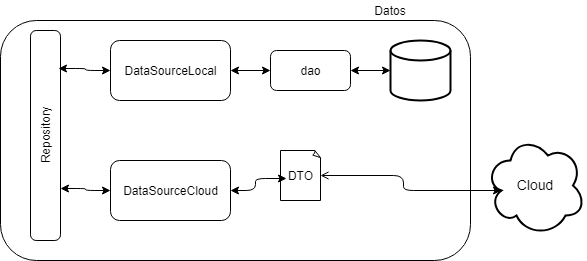
\includegraphics[width=0.7\linewidth]{Desarrollo/Arquitectura/imgs/iagram.png}
\caption{Capa de datos Android}
\end{figure}

\item \textbf{ Common:} Y por último esta el módulo common, aquí es donde se ponen las clases u utilidades que comparten todos los módulos, y por tanto aquí es donde se definen los modelos de la app, que son comunes en las capas.
\end{enumerate}

\newpage
\subsubsection{BackEnd}

Para el backend se utiliza otra combinación de tecnologías

\begin{figure}[h!]
\centering
\begin{subfigure}{.1\textwidth}
  
\includegraphics[width=0.5\linewidth]{Desarrollo/Arquitectura/imgs/JHipster-logo.png}
\end{subfigure}%
\begin{subfigure}{.1\textwidth}
  
\includegraphics[width=0.7\linewidth]{Desarrollo/Arquitectura/imgs/spring.png}
\end{subfigure}
\begin{subfigure}{.1\textwidth}
  
\includegraphics[width=\linewidth]{Desarrollo/Arquitectura/imgs/java.jpg}
\end{subfigure}
\begin{subfigure}{.1\textwidth}
  
\includegraphics[width=0.9\linewidth]{Desarrollo/Arquitectura/imgs/docker_facebook_share.png}
\end{subfigure}
\end{figure}

Su core es en Java (1.8), se utiliza una herramienta que es Jhipster, y para el despliegue en los ambientes se utiliza docker. \\

Se utiliza una arquitectura de tres capas, en donde se tiene el Api con toda la funcionalidad del servicio REST, la capa de servicio, en donde está toda la lógica del negocio, y la capa de datos en la cual tenemos toca la comunicación con las bases de datos, se utiliza el patrón Dao y la librería de Hibernate.

\subsubsection{FrontEnd Web de Administración}

\begin{figure}[h!]
 \centering

\includegraphics[width=0.1\linewidth]{Desarrollo/Arquitectura/imgs/Angular_full_color_logo.png}
\end{figure}

Se utiliza la versión 5 de angular, y se implementa toda la parte de la administración de los valores o parámetros de la página web. A través de esta herramienta, se puede administrar:

\begin{itemize}[noitemsep]
\item Grupos Musicales
\item Categorías
\item Imágenes
\item Solicitud de cotización
\item Usuarios
\item API
\item Logs
\item Auditoría
\item Estado del servidor
\item Métricas
\end{itemize}

\newpage

\subsection{Lógica}
\begin{figure}[h!]
 \centering
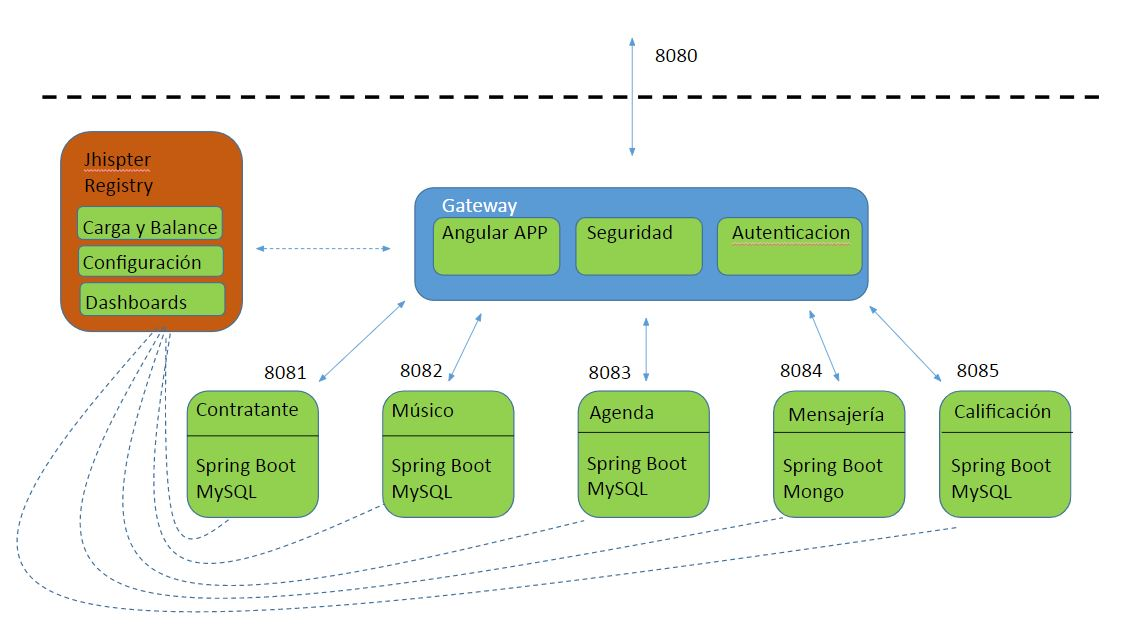
\includegraphics[width=\linewidth]{Desarrollo/Arquitectura/imgs/servicios.JPG}
\caption{Diagrama de Logica del backend}
\end{figure}
Por medio de JHipster Registry se asociarán los servicios de la aplicación; además de permitir la administración de los mismos. El core de la aplicación se subdivide en cinco servicios que administran la funcionalidad que llevan por nombre. Como capa superior se encuentra el API Gateway que presenta las las centraliza los servicios y se encarga de la seguridad y autenticación a la aplicación.
a continuación se detallaran los servicios enunciados en el diagrama:\\
\begin{itemize}

\item \textbf{Contratante:} encargado de la publicación de los datos del rol que lleva por nombre; Este servicio deberá permitir la administración de la cuenta del usuario autenticado dando la posibilidad de actualizar crear y eliminar las características y los datos persistidos en la base de datos. Se expondrá en el puerto 8081.
\item \textbf{Músico:} este servicio actuará de forma similar al contratante en cuanto a la administración de los datos de la cuenta, adicionalmente preferencias de servicios y descripciones de servicios ofertados. Se expondrá en el puerto 8082.
\item \textbf{Agenda:} la sincronización de los datos de músico y contratante se verán afectados en este servicio que adicionalmente administra datos de calendario para la ejecución de servicios contratados, preferencias y acuerdos entre los actores de la aplicación. Se expondrá en el puerto 8083.
\item \textbf{Mensajería:} con este componente se mediará la comunicación entre usuarios, debe permitir la generación de notificaciones que serán de creación, consulta. Se expondrá en el puerto 8084.
\item \textbf{Calificación:} Este servicio validará la relación generada entre el contratante y el músico para finalizar con la posibilidad de ambos actores de retroalimentar la experiencia. Los datos manipulados en esta capacidad serán creados, modificados y consultados. Se expondrá en el puerto 8085.
\end{itemize}


\subsection{Física}
\begin{figure}[h!]
 \centering
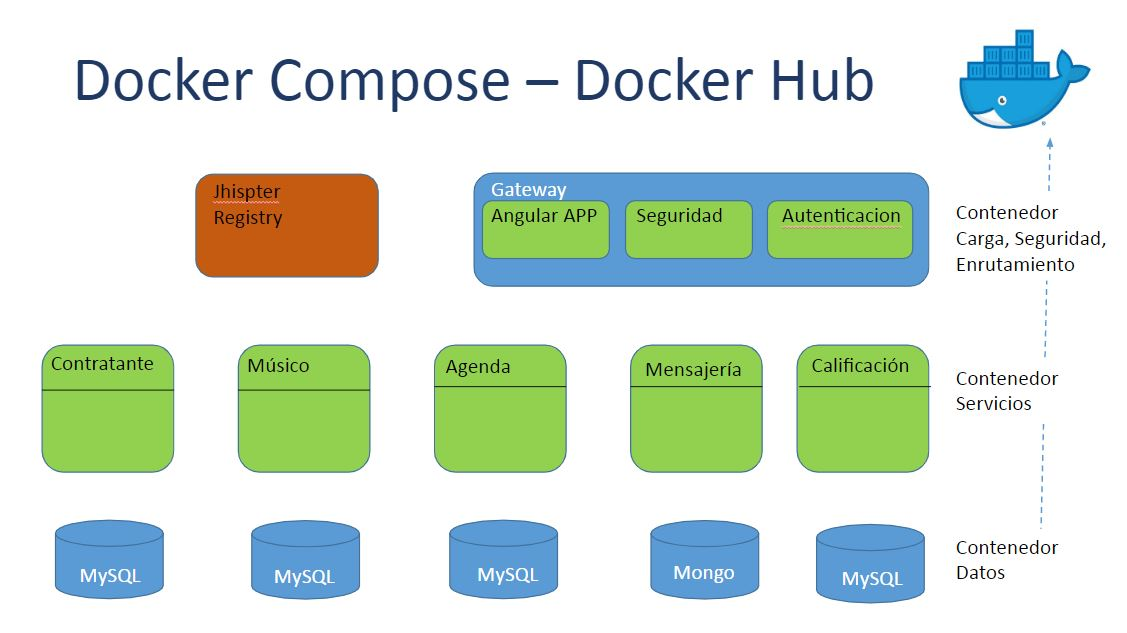
\includegraphics[width=\linewidth]{Desarrollo/Arquitectura/imgs/contenedores.JPG}
\end{figure}
Se aplicará la tecnología Docker para producir los ambientes, desarrollo, prueba, producción cada uno con los contenedores presentados en el diagrama, publicando la configuración en DockerHub y realizando los ajustes necesarios para sincronizar los diferentes componentes a través de Docker Compose

\subsection{Seguridad}